\documentclass{report}
\usepackage{graphicx, subfigure}
\usepackage{mathtools}
\usepackage{hyperref}
\usepackage{float}
\usepackage[section]{placeins}
\usepackage{listings}

\lstset{frame=tb,
    language=Python,
    basicstyle={\small\ttfamily},
    breaklines=true,
    breakatwhitespace=true,
    tabsize=3
}

\begin{document}

    \title{Phase Field Simulations}
    \author{Bruce Berry}
    \maketitle

    \section{Introduction}
    This report details the simulation of various molecular scale events.  The Molecular Dynamics (MD) method is used to simulate inter-particle interactions.

    \section{Background}

    \section{Methods}
        \begin{figure}[!htb]
            \label{fig:applied-stress}
            \centering
            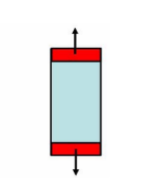
\includegraphics[width=0.4\textwidth]{applied-stress.png}
            \caption{The stress Initial Condition.}
        \end{figure}

        \subsection{Copper Nanowire}
        Of interest is the simulation of a copper Nanowire's reponse to deformation.  Simulations were carried out using Nanohub's Nanowire Tensile Deformation Lab (NTDL) module.  A lattice of atoms were generated of size 20 x 20 x 130 \AA. As per the assignment's direction, the NTDL parameters were set to 8 x 8 x 36 to produce this initial condition.  The structure was set to be a free surface in each direction, with a tensile force applied to each end ~\ref{fig:applied-stress}.  The tensile stress was implemented by applying a displacement of 0.02 \AA every 20 simulation time steps. 30,000 time steps were performed.  The simulation was carried out a second time, with the cross sectional area doubled (40 x 40 x 130 \AA).

          

    \section{Results}



\end{document}
